%!TEX root = ../project3.tex
\section{Konzept}
Der Evolutionäre Algorithmus mutiert das Individuum. Im konkreten ist das Individuum ein neuronales Netz. Das Netz wird durch den Algorithmus auf bestimmte Start Konstellationen des Simulators hin trainiert. Durch verschiedene Anpassungen der Parameter des Algorithmus kann der gesamte Vorgang modifiziert werde um zum Beispiel das Netz zu vergrößern oder Parameter der Mutation anzupassen.

\section{Repräsentation}
Die Strategie wird durch ein künstliches neuronales Netz (KNN) entschieden, welches auf bestimmte Eingabewerte hin Entscheidungen trifft und die Verteilung der Aktionspunkte am Simulator vornimmt. Das neuronale Netz besteht im wesentlichen aus einen Eingabeschicht mit 9 Neuronen und einer Ausgabeschicht mit 6 Neuronen. Zwischen der ein und Ausgabe sind frei konfigurierbare Layer angeordnet mit gleicher Breite. 


\begin{figure}[h!]
\begin{center}
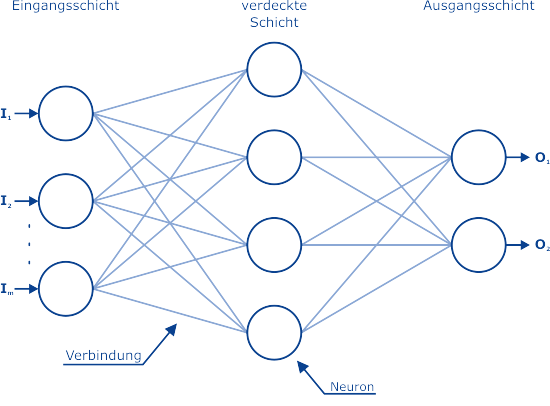
\includegraphics[scale=1.5]{images/knn}
\caption{typischer Aufbau eines KNN;\textit{ Quelle: http://www.lfi.rwth-aachen.de/}}
\label{KNN}
\end{center}
\end{figure}

Die Anzahl ist auch Variabel so kann diese von 1 bis n festgelegt werden. Diese Schichten werde verdeckte Schicht genannt und sind im Implementierten Individuum voll-vernetzt. Das bedeutet ein Neuron der Schicht \textit{n} gibt seine Informationen an jedes von \textit{n+1} weiter. Schematisch wird dies in (Abb. \ref{KNN}).

\section{Evolutionsare Operatoren}
Ein Neuron des Netzes wird über 2 Parameter gesteuert. Eine Dämpfung ein Gewichtung. Ein Netz aus 5 Schichten jeweils mit 5 Neuronen hat somit 50 Werte, welche angepasst und mutiert werden müssen. Für die Mutation wird dafür die Selbstadaptive-EP-Mutation verwendet. Diese kann im Detail hier \citep[S.146]{Weicker2007} nachgelesen werden. Eine kurze Beschreibung:

Zu jedem Neuron und dessen 2 Werte existieren zusätzlich 2 Werte welche die Änderungen am Neuron bestimmen. Zunächst verändert die Mutation diese Anpassungsparameter. Nun werden die eigentlichen Werte des Neurons mutiert, hierfür wird der zuvor mutierte Anpassungsparameter einbezogen. Das Ergebnis aus der Mutation sind neue Anpassungsparameter für das Neuron und dessen Gewichtung und Dämpfung.

Der Evolutionsare Operatoren besteht nur aus einer Mutation er hat keine Rekombination.

\section{Selektionsdruck}
Die Population des Evolutionsare Algorithmus ist variable, sie besteht zu beginn aus \textit{x} Eltern Individuen. Diese Werden der Gesamtpopulation hinzugefügt. Die Eltern werden nun mutiert, es entstehen \textit{x} Kind Individuen, welche ebenso der Gesamtpopulation hinzugefügt werden, diese hat nun einen Umfange von \textit{2x} Individuen.

Die Selektion wählt nun die x Besten Individuen aus der Population aus welche die neunen Elternindividuen werden.

\section{Gutsbewertung}
Die Gütebewertung der Individuen und deren Strategie wird durch die überlebte Rundenanzahl realisiert. Für gleiche Individuen (überstandene Runden) kann eine weitere Bewertung durch die Bilanz erfolgen.

\section{Simulationsszenarien}
Als Ausgangsimulation wurde verwendet \ensuremath{[8, 1, 12, 13, 4, 10, 20, 21, 0]}. Auf Basis dieser wurden 50 Zufällige Situationen erzeugt, welche sich um ein \ensuremath{\epsilon \approx 1}  zum Ursprung unterscheiden können. Ein Paar Beispiele: 
\begin{itemize}
\item\ensuremath{[7,	1,	13,	12,	4,	9,	20,	22,	2]},
\item\ensuremath{[8,	2,	12,	13,	5,	11,	20,	21,	1]},
\item\ensuremath{[8,	3,	12,	13,	4,	10,	20,	21,	0]},
\item\ensuremath{[7,	2,	11,	12,	3,	9,	19,	20,	1]},
\item\ensuremath{[7,	3,	12,	12,	5,	11,	21,	21,	1]},
\item\ensuremath{[9,	1,	11,	13,	5,	9,	21,	21,	0]}.
\end{itemize}

Anschließend wurde das Individuum gegen eine Auswahl von 5000 Simulationen mit \ensuremath{\epsilon \approx 5} zur Standartvorgabe getestet.

\section{Effizienz}
Das Individuum besteht aus einem Netz mit 8 Layer davon 6 Verdeckte-Layer mit jeweils 16 Neuronen. Die Laufzeit betrug circa eine halbe Stunde und es mussten fast 1000 Generationen erzeugt werden. Die insgesamt wurden über 20 solche Tests gemacht um ein perfektes Individuum zu erzeugen.

Ausschlaggebend für den Erfolg ist jedoch auf welchen Startzustand des Simulators hin optimiert werden soll. Sehr große Startbereiche, Bereiche mit einem großen Epsilon benötigen viel länger und mehr Generationen und erreichen auch nicht die vorgegebene Konditionieren, dass alle Startkonstellationen zu einer maximalen Rundenanzahl von 30 Runden führen.

\section{Fazit}
Die Strategie welche im Neuronalen Netz erfasst ist abhängig von der Größe des Netzes. Ein hinreicht großes Netz ist sicher in der Lage für alle Startkonstellationen eine Strategie auszuführen, welche 30 Runden im Simulator überlebt. Schwachpunkt ist die zu Langsame Mutation die Dauer für die Generierung solch eines Individuums ist enorm.

Ein Knackpunkt ist die Implementierung des Pseudozufallszahl-Generator von Java er verbraucht mit Abstand die meiste Laufzeit in der Mutation. Eine effizientere Methode würde die Mutation beschleunigen. Insgesamt wurde ein vielfaches mehr Zeit für die Bearbeitung und Implementierung des Projektes verwendet als angesetzt wurde.

Eine zusätzliche Testumgebung lädt ein beliebiges Individuum erzeugt eine beliebige Anzahl von Test Simulationen und lässt das Individuum gegen den Simulator antreten. Zehntausend Testfälle werden in weniger als 10 Sekunden abgearbeitet und ausgewertet werden. Sämtlicher Code liegt dieser Ausarbeitung bei und kann frei verwendet werden.